\documentclass[a4paper ,12pt, onecolumn]{article}
\usepackage[utf8]{inputenc}
\usepackage[spanish]{babel}
\usepackage[hidelinks]{hyperref}
\usepackage{graphicx}

\usepackage{pgfgantt}
\usepackage{xcolor}
\usepackage[utf8]{inputenc}


\graphicspath{ {./images/} }
\begin{document}
\title{Sistemas de posicionamiento de objetos mediante tecnología Bluetooth Low Energy Beacon }
\author{Rubén Arce}
\date{\today}
\maketitle
\cleardoublepage
\tableofcontents
\cleardoublepage
\section{Memoria descriptiva}
    Antecedentes, objeto, normativa, reglamentación
    Extensión máxima de 30 páginas + anexos 60
    Defensa de 20 min  40
    \subsection{Antecedentes y objeto del proyecto}
        Este proyecto surge como respuesta a la necesidad de poder localizar un número elevado de equipos en 
        constante movimiento con exactitud en un espacio cerrado.
        \paragraph{}
        Se pretende conseguir los siguientes objetivos:
        \begin{enumerate}
            \item Estudio sobre las distintas alternativas para llevar a cabo este tracking de objetos de una forma
            sencilla y sin requerir de una inversión grande.
            \item Análisis de las tecnologías existentes para la monitorización en interiores.
            \item Estudio del parámetro RSSI como medida de la potencia de una señal y cálculo de la distancia entre equipos.
            \item Desarrollo de un sistema de visualización mediante un mapa sobre el que poder ver los equipos en movimiento.
            \item Diseño de hardware específico para la aplicación requerida.
            \item Programación tanto del equipo emisor como del receptor así como del algoritmo de visualización.
            \item Pruebas de campo y comprobación del rendimiento del equipo.
        \end{enumerate}
        \paragraph{}
        Una vez fijado el alcance del proyecto se puede empezar a planificar el mismo y buscar la mejor solución 
        posible, por ello surgen los siguientes objetivos derivados de los primeros para poder sacar el producto 
        al mercado:
        \begin{enumerate}
            \item Precio muy competitivo.
            \item Producto estándar y de fácil aplicación.
            \item Sencillez de instalación por un usuario no técnico.
            \item Poco o nulo manteniminto.
            \item Producto seguro y que preparado para superar los marcados UL y CE.
        \end{enumerate}
    \subsection{Ambito de aplicación}
        El tracking de objetos en espacios cerrados está incrementando su popularidad debido a que es una 
        arma de propaganda muy poderosa que demandan los grandes centros comerciales para llevar a cabo estudios de marketing
        y poder analizar el comportamiento de los clietes.
        \paragraph{}
        Además de esta aplicación el mayor nicho de mercado es aplicado a no tener que tocar objetos para interactuar con ellos, 
        esto teniendo en cuenta los tiempos que corren es una necesidad de numerosas empresas privadas, ayuntamientos 
        y empresas estatales.
        \paragraph{}
        A modo de resumen se engloban los principales ámbitos de aplicación de esta tecnología:
        \begin{enumerate}
            \item Marketing: Estudios de mercado y de necesidad de los clientes. Elaboración de un "heat map", o mapa 
            de las zonas con más afluencia de gente.
            \item Seguridad: Tan solo los empleados con autorización y proximidad podrán llevar a cabo acciones,
            esto tiene sentido a la hora de no tener que dar una llave a cada empleado que pueda duplicarse.
            \item Vandalismo: Conociendo la localización de los equipos dentro de un local cerrado en el momento 
            en el que se deja de situar un elemento se puede dar la voz de alarma ante un robo.
            \item Propaganda y nueva forma de publicidad: Activar acciones en función de la localización en determinados
            puntos de interés permite llevar a otro nivel las ideas de los publicistas.
        \end{enumerate}
        Vemos por tanto que hay numerosas aplicaciones y demanda de este producto tecnológico, es por ello por lo que se 
        procede a explorar cual es la forma más adecuada para llevarlo a cabo e implementarlo.
    \subsection{Análisis de soluciones al tracking de objetos}
        Se plantean dos problemáticas, en primer lugar se busca llevar a cabo el seguimiento de elementos en movimiento, y por el otro 
        está el enviar esta información de alguna forma al sistema correspondiente para que lleve a cabo el análisis de los datos. Esta
        última acción es esencial en el proceso, es lo realmente interesante desde el punto de vista del cliente final de esta tecnología.
        En lo que respecta a la obtención de datos de posición relativa de objetos o personas se presentan las siguientes opciones:
        \subsubsection {Wifi}
            La posibilidad de llevar a cabo el tracking mediante la escucha de wifis es una opción, para ello sería
            necesario en primer lugar que se colocara un móvil en cada uno de los objetos a identificar. Esto es aceptable 
            en el caso de monitorización de personas pero inasumible para objetos.
            \paragraph{}
            El procedimiento consistiría en llevar a cabo un barrido de direcciones MACs que generan los móviles cuando tienen el wifi activado,
            es decir que este sistema no funcionaría en el caso de que una persona lleve puestos los datos del móvil únicamente.
            \paragraph{}
            Otra desventaja es el hecho de que al tener un equipo buscando wifis la información personal del propietario, es decir, localización,
            fecha, hora a la que se intentó conectar y la dirección MAC que identifica y relaciona un móvil a una persona queda expuesta.
            Se han de tener en cuenta la política de privacidad vigente, empleando esta tecnología para llevar a cabo el tracking se inclumpliría.
            \begin{center}
                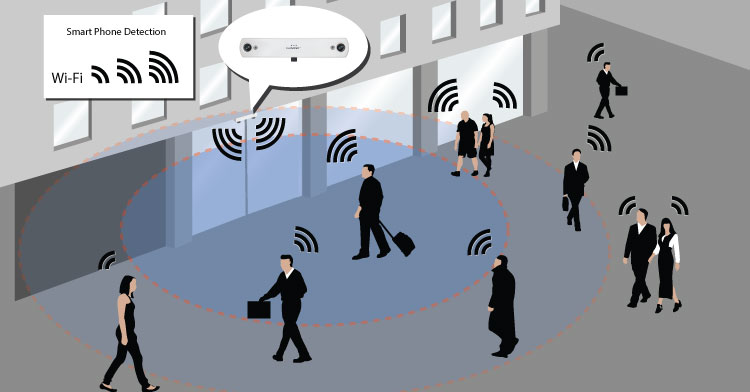
\includegraphics[scale=0.3]{WifiCounting.jpg}
            \end{center}
            La única solución al problema es que se ha de pedir permiso formal a la persona para poder llevar a cabo
            el tratamiento de sus datos, cosa que es dificil puesto que se desconoce quien va a llevar a cabo el uso del equipo.
            \paragraph{}
            El artículo 29 de privacidad de datos de la comunidad europea dice lo siguiente:
            “WiFi-tracking, depending on the circumstances and purposes of the data collection, such tracking under the GDPR is likely
            either to be subject to consent, or may only be performed if the personal data collected is anonymised”
            Es por ello por lo que aunque se tendrá en cuenta como opción hay numerosos puntos en contra de implementar un sistema como este.
        \subsubsection {GPS}
            La tecnología por excelencia para llevar a cabo el seguimiento de objetos o personas es el GPS, la principal desventaja
            que presenta es el elevado consumo energético comparado con el wifi o el bluetooth.
            \paragraph{}
            Mantener un módulo GPS encendido y pretender llegar a una autonomía de años es a día de hoy
            imposible, es por ello por lo que o se emplea un teléfono móvil para llevarlo a cabo, cosa inviable si se pretende 
            monitorizar objetos  y no personas en movimiento, o el tiempo de refresco de los datos ha de ser muy lento, del orden de horas,
            cosa de nuevo inviable para la aplicación que se tiene entre manos.
            \paragraph{}
            Se ha de tener en cuenta también el aumento de precio que supondría un módulo GPS sumado a la antena que lleva consigo de 
            dimensiones nada despreciables. 
            Es por ello por lo que esta tecnología se tendrá en cuenta pero no es la más adecuada para la problemática presente.
        \subsubsection {Bluetooth Low Energy - Beacon}
            Bluetooth 
            Emisión desde los -20 dBm (0.01 mW) hasta los +20 dBm (100 mW). Cuanta mayor potencia de emisión mayor consumo energético
            del dispositivo pero también conseguiremos una mayor distancia.
            Existen varios tipos de beacons:
            \begin{enumerate}
                \item iBeacon: Fue la primera tecnología BLE Beacon desarrollada por Apple, permite leer y emitir en modo 
                broadcast para cualquier dispositivo que disponga de Bluetooth low energy. Es un protocolo propietario, es 
                decir es un estandar cerrado. 
                Los iBeacons disponen de los siguientes identificadores:
                \begin{itemize}
                    \item UUID: Se basan en enviar el indentificador único de dispositivo, una cadena de
                    carácteres de 16 bytes que permite caracterizar a caba equipo.
                    \item Major: Número entero de 0 a 65535, se usa para identificar grupos, un ejemplo sería 
                    asignar un Major común para todos los beacons de una misma planta o habitación.
                    \item Minor: Es también un número entero de 0 a 65535 que se emplea para distinguir un beacon
                    específico dentro de un grupo, entendiéndose como grupo aquellos beacons con mismo valor de Major.
                \end{itemize}
                \begin{center}
                    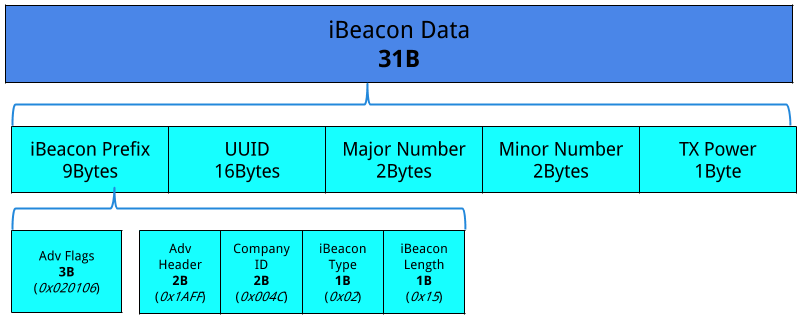
\includegraphics[scale=0.4]{tipos_beacon_ibeacon.PNG}
                \end{center}
                \item Eddystone: Creado por Google es un protocolo de código abierto. A diferencia del protocolo anterior este 
                permite transmitir:
                \begin{itemize}
                    \item URL: Un url propio de una web, de esta forma se evita la necedad de tener que contar con una app instalada.
                    \item UID: Similar al UUID del iBeacon, este parámetro identifica al beacon y permite llevar acciones individuales.
                    \item TML: Permite enviar información relativa al beacon como por ejemplo el porcentaje de batería o valores de sensores.
                \end{itemize}
                \begin{center}
                    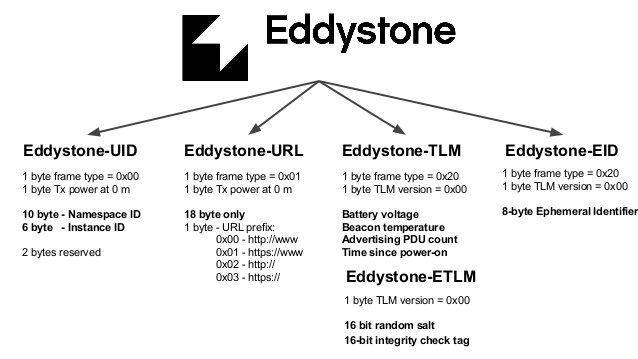
\includegraphics[scale=0.4]{tipos_beacon_edison.PNG}
                \end{center}
                \item AltBeacon: Es un protocolo de código abierto que surge como resultado de las incompatibilidades de las dos 
                tecnologías anteriores, la ventaja principal es que permite más flexibilidad de modificaciones así como compatibilidad 
                entre sistemas operativos.
    \subsection{Análisis de soluciones a la subida de datos}
        Una vez exploradas las opciones de posicionamiento de los equipos se llevará a cabo el estudio de posibilidades de subida de estos datos
        a la nube, es por ello por lo que se contemplar varias opciones:
        \subsubsection {MQTT}
            MQTT es un protocolo estándar aplicado principalmente al IoT (Internet of Things). Está basado en publicación y 
            suscripción con un servicio de mensajería push, los mensajes se publican el topics en los que los distintos 
            dispositivos se encuentran escuchando.
            La base de la comunicación es el Broker, encargado de dar soporte a todos los topics, los clientes inician una 
            conexión TCP/IP con él que se mantiene abierta constantemente hasta que el cliente la finalize. Se emplean los puertos
            1883 y 8883 empleando seguridad TLS.
            Cada mensaje tiene un QoS (Quality of service), es el mecanismo de calidad del servicio, o lo que es lo mismo es la forma de
            gestionar la robustez de los mensajes entre clientes ante los fallos de conectividad.
            \begin{itemize}
                \item QoS 0: Envio una única vez
                \item QoS 1: Menaje enviado hasta que se garantiza que se entrega.
                \item QoS 2: Garantizado que cada mensaje se entrega al suscriptor por una única vez.
            \end{itemize}
            Esta es una opción para que los equipos que escuchan a los beacons y envian la información a un mismo
            topic en el que el sistema de visualiación está escuchando.
        \subsubsection {HTTP post}
            A través del protocolo de transferencia de hipertexto se puede llevar a cabo una petición POST, consiste en que
            un servidor acepte los datos recibidos por el microcontrolador.
            La ventaja es que con el HTTP Post solo se mantiene la conexión abierta al hacer la conexión, luego se desconecta hasta 
            la siguiente vez en la que se vuelvan a publicar datos. Otra ventaja es que mediante peticiones se pueden llevar a 
            cabo varias a distintos servidores, por el contrario con MQTT solo se puede enviar información a aquellos que estén
            suscritos al mismo tópic.
            El principal inconveniente es que está demostrado que en una red 3G una petición post es del orden de 93 veces
            más lenta que un mensaje MQTT, con el consiguiente consumo energético que esto conlleva. Otro inconveniente es el hecho 
            de que se requiera de un servidor con una API o endpoint constantemente escuchando a los distintos posts.
        \subsubsection {ESP Now}
            Se plantea la opción de que no todos los equipos que escuchan a los beacons no tengan internet, es por ello por lo 
            que se plantéa llevar a cabo una red de elementos que escuchan y que envian a un único concentrador encargado de enviar
            esta información a internet por cualquier otro método.
            Es decir, se contempla la posibilidad de establecer una red de elementos que escuchan, para ello se emplea 
            un protocolo de comunicación rápido denominado ESP-NOW, este tiene las siguientes características:
            \begin{itemize}
                \item Encriptación de las comunicaciones.
                \item Hasta 250 Bytes de payload o mensaje a enviar.
                \item Rapidez de comunicación entre esps
            \end{itemize}
            \paragraph{}
            La idea sería la siguiente:
            \begin{enumerate}
                \item El equipo que lleva a cabo el barrido y búsqueda de beacons escanea e intenta conectarse a 
                internet por wifi.
                \item Si lo consigue publica los datos, en el caso de que falle enviará por ESP NOW la información
                que no puede subir a internet a otro equipo en su misma red que si que pueda.
                \item Este segundo hará lo mismo hasta que finalmente haya uno que si que pueda subir estos datos.
            \end{enumerate}
            \begin{center}
                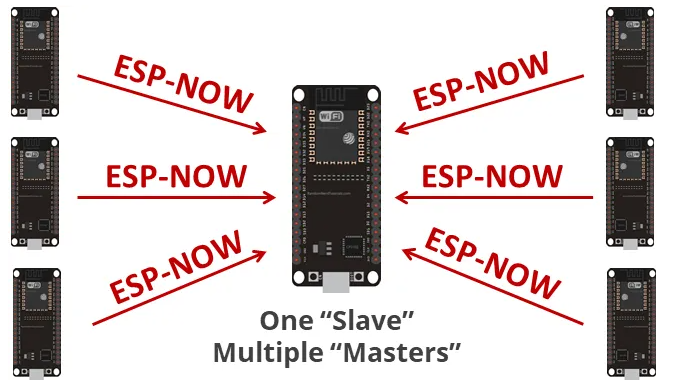
\includegraphics[scale=0.4]{espnow.png}
            \end{center}
        \end{enumerate}
    \subsection{Resultados finales}
        Una vez analizadas las dos problemáticas y las distintas soluciones a cada una de ellas se ha confeccionado la siguiente tabla 
        en la que se puede ver una comparativa entre cada una de ellas.

        Por un lado está la forma en la que poder medir las distancias de los equipos con respecto a los equipos que escuchan,
        se contemplaban las siguientes opciones:
        \begin{center}
            \begin{tabular}{|c | c| c| c| c |} 
            \hline
            Tecnología  & Coste  & Complejidad & Distancia & Consumo energético \\ [0.5ex] 
            \hline
            GPS& Elevado& Baja & Ilimitada& Muy alto\\
            Wifi& Medio& Media & ~ 100 m & Alto\\ 
            Bluetooth& Bajo& Media & ~ 100 m & Muy bajo\\ 
            \hline
            \end{tabular}
        \end{center}   
        El claro ganador en este caso es el Bluetooth debido principalmente al precio que supondría llevar a cabo una red de estas 
        características además del consumo energético tan bajo hace que el mantenimiento de los equipos sea casi inexistente.
        \paragraph{}
        Recordemos que una de las premisas iniciales era que los equipos requerieran de poco cuidado por parte del cliente, empleando
        esta tecnología se puede conseguir que solo sea necesario cambiar una pila una vez al año.
        \paragraph{}
        En lo que respecta a la comunicación de estos datos de distancia entre equipos a internet se ha reunido de nuevo en la 
        siguiente tabla un resumen con las opciones y los puntos a favor y en contra de cada una de las tecnologías.
        \begin{center}
            \begin{tabular}{||c | c| c| c||} 
            \hline
            Tecnología  & Velocidad de datos & Coste & Complejidad \\ [0.5ex] 
            \hline
            MQTT& Elevada  & No & Baja\\
            HTTP POST& Baja & Medio & Baja\\ 
            ESP NOW& Media & No & Alta\\ 
            \hline
            \end{tabular}
        \end{center}   
        La elección en este caso está mucho más ajustada, en el caso de que se pueda conectar a todos los equipos que 
        escuchan a internet el ganador será la opción de MQTT puesto que la forma más facil de llevar a cabo el envio de datos.

        En el caso de que no llegue la señal wifi a todos los puntos en los que se decida llevar a cabo el tracking de objetos 
        surge un problema puesto que perderemos esos datos, la solucion es hacer que este equipo, que no tiene conexión a internet,
        envie los datos por ESP NOW a otro que si que sea capaz de subir tanto su información como la de su compañero al broker por MQTT.

        Puesto que se pretende llevar a cabo un sistema válido para toda la casuística de instalaciones se han contemplado ambas opciones
        y la implementación real llevará a cabo los dos métodos.
        
        Es decir que la única opción desechada ha sido la conexión directa con un servidor mediante HTTP debido a que, en primer
        lugar sería necesario programar un servicio que escuchara en este endpoint y luego sería necesario hostearlo 
        para que disponga de una IP pública estática y sea accesible desde cualquier parte del mundo.
    \subsection{Planificación}
        \paragraph{}
        Para sintetizar el proceso de desarrollo del proyecto técnico se empleará un diagrama GANTT: 
        \begin{itemize}
            \item Fase 1: Analisis de la situación.
            \item Fase 2: Definición de la problemática.
            \item Fase 3: Búsqueda de soluciones y alcance del proyecto.
            \item Fase 4: Desarrollo de hardware acorde a especificaciones.
            \item Fase 5: Programación del receptor de los datos.
            \item Fase 6: Programación del hardware.
            \item Fase 7: Pruebas de campo.
            \item Fase 8: Depuración tanto de programación como de bug en hardware.
            \item Fase 9: Evolución del equipo en instalación.
            \item Fase 10: Evaluación de producto y producción masiva.
        \end{itemize}
        \begin{center}
            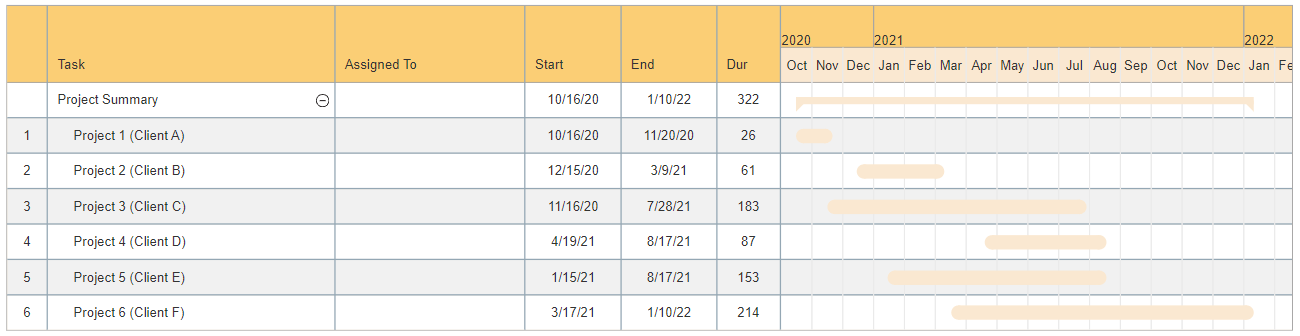
\includegraphics[scale=0.35]{gantt.PNG}
        \end{center}
        https://online.visual-paradigm.com/ tiene buena pinta para hacer esto
        
\section{Memoria justificativa}
    \subsection{Cálculos justificativos de la instalación}
        En este apartado de llevará a cabo el estudio de la viabilidad del proyecto desde el punto de vista
        técnico, para lo cual se contemplará un estudio del rssi como forma de medir distancia, un análisis 
        de la previsión energética de los equipos, un análisis del las frecuencias y ganancias de las antenas 
        empleadas.
    \subsection{Cálculo de distancia por RSSI}
            \subsubsection{Rssi}
                \paragraph{}
                El RSSI (Received signal strength indicator) es un indicador de la energía o potencia recibida en un mensaje de radio, 
                está asociado con la atenuación de la señal, cuanto más pequeña es su valor menor atenuación. Este valor está 
                presente no solo en Bluetooth sino también en el Wifi (2,4 GHz) o en las bandas de radio industriales, científicas y médicas,
                las denominadas ISM (desde 433MHz a 458.5MHz y desde 860MHz a 960MHz)
                \paragraph{}
                De las muestras obtenidas se puede concluir que se puede llegar a estimar la distancia a partir de los valores
                de rrsi con un error que disminuye cuanto más alejados son los elementos a medir. 
                \paragraph{}
                Los rangos del RRSI se obtiene bien por aproximaciones teóricas o bien por experimentación, esto es debido a que 
                es fuertemente alterado por las condiciones del medio en el que se encuentre. Es importante mencionar también que
                este parámetro es medido a través de un hardware que rara vez tiene un comportamiento idéntico.
                \paragraph{}
                Los modelos de cálculo del RRSI se basan en la pérdida de señal en el espacio, como sabemos la potencia de la señal
                disminuye con el cuadrado de la distancia. Esta ecuación de Friis para la transmisión libre en el espacio espacio es 
                una fórmula teórica, existen aproximaciones obtenidas por métodos empíricos:
                \begin{equation}
                    P_L(d) [dB] = P_L(d_0) [dB] + 10n *\log_{10} \frac{ d_i }{d_0} 
                \end{equation}
                \paragraph{}
                Siendo PL (d0) la pérdida de propagación a 1 metro y n es una constante que depende del medio, será igual
                a 2 si se encuentra en el espacio libre sin obstáculos ni reflexiones o dispersiones de señal.
                \paragraph{}
                Para calcular este parámetro 'n' se ha de aplicar la siguiente fórmula, como podemos ver para llevar a cabo el 
                cálculo se han de tomar valores empíricos de potencias:
                \begin{equation}
                    n = \frac{ P_L(d_i) - P_L(d_0) }{10n*\log_{}\frac{d_i}{d_0}}
                \end{equation}
                \paragraph{}
                Por lo tanto, y una vez obtenidos los valores de potencia a distintas distancias podemos obtener la ganacia
                de la señal recibida:
                \begin{equation}
                    RRSI [dBm] = -10n*\log_{10} d+ A[dBm]
                \end{equation}
                \paragraph{}
                Disponiendo ya del valor de la constante de pérdidas, d, calculado con la ecuación (2) y los valores
                de rssi medidos desde la antena receptora a 1 metro de distancia, A, podemos obtener:
                \begin{equation}
                    d= 10^\frac{-(RRSI - A)}{10n}
                \end{equation}
                Llevados a cabo los cálculos por parte del equipo que escucha a los distintos beacons podemos calcular la distancia 
                real a cada uno de ellos. En el caso de que se solapen y dos receptores escuchen el mismo beacon será necesario
                llevar a cabo el proceso de trilateración expuesto a continuación.

                Para comprobar la fluctiación del parámetro del rssi se ha llevado a cabo la toma de este valor a los largo de un 
                periodo de tiempo largo y estos son lo resultados a 2 metros y a 3 metros:
                \begin{center}
                    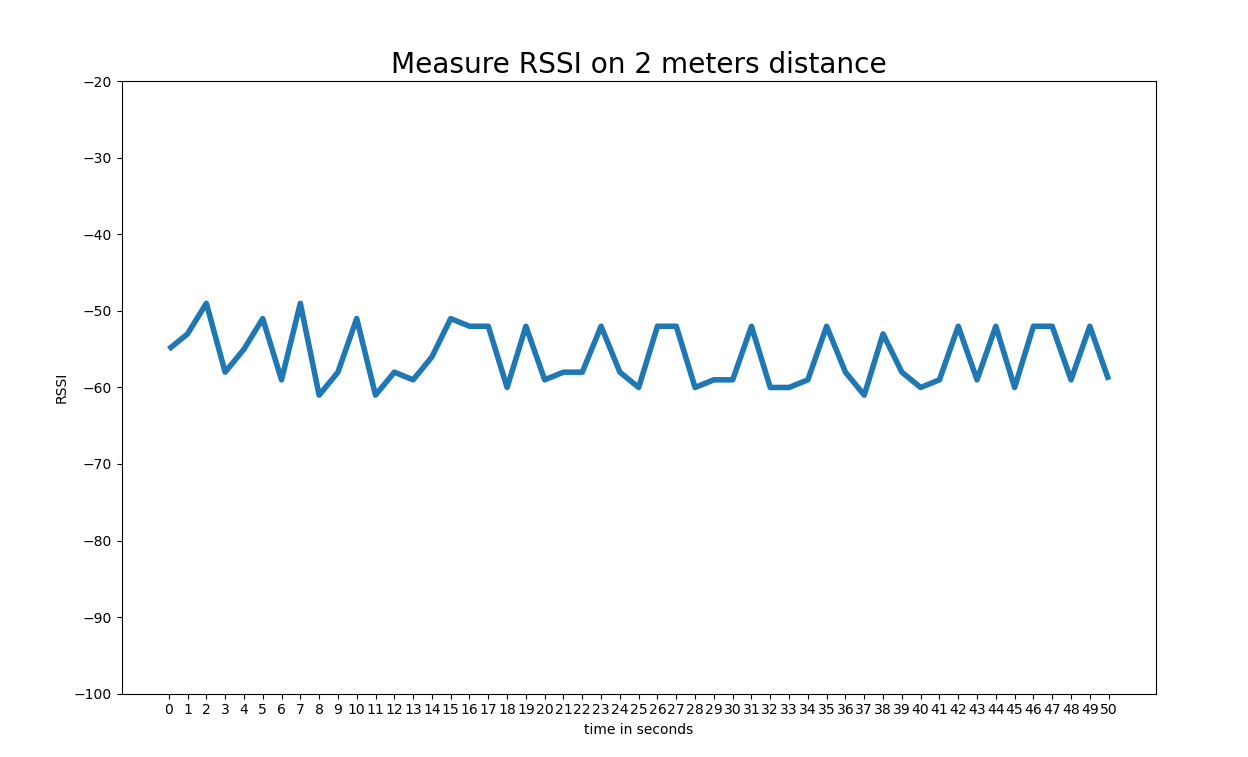
\includegraphics[scale=0.35]{1_beacon_2_meters.PNG}
                    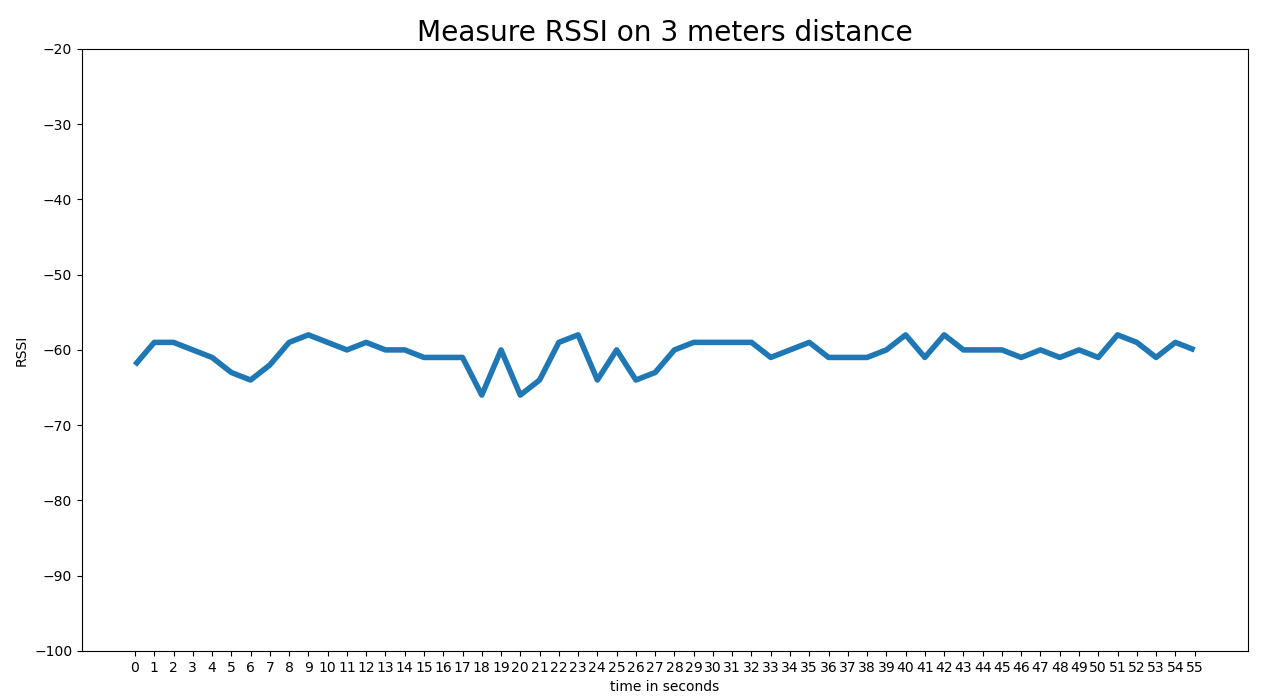
\includegraphics[scale=0.3]{1_beacon_3_meters.PNG}
                \end{center}
                Podemos ver que hay pequeñas fluctiaciones y es por ello por lo que será necesario implementar un sencillo filtro para
                evitar el ruido electromagnético que hemos visto anteriormente.
                \paragraph{}
                Otra prueba llevada a cabo ha sido la de incrementar el número de iBeacons y situarlos a la misma distancia del 
                equipo que escucha, los resultados son los siguientes:
                \begin{center}
                    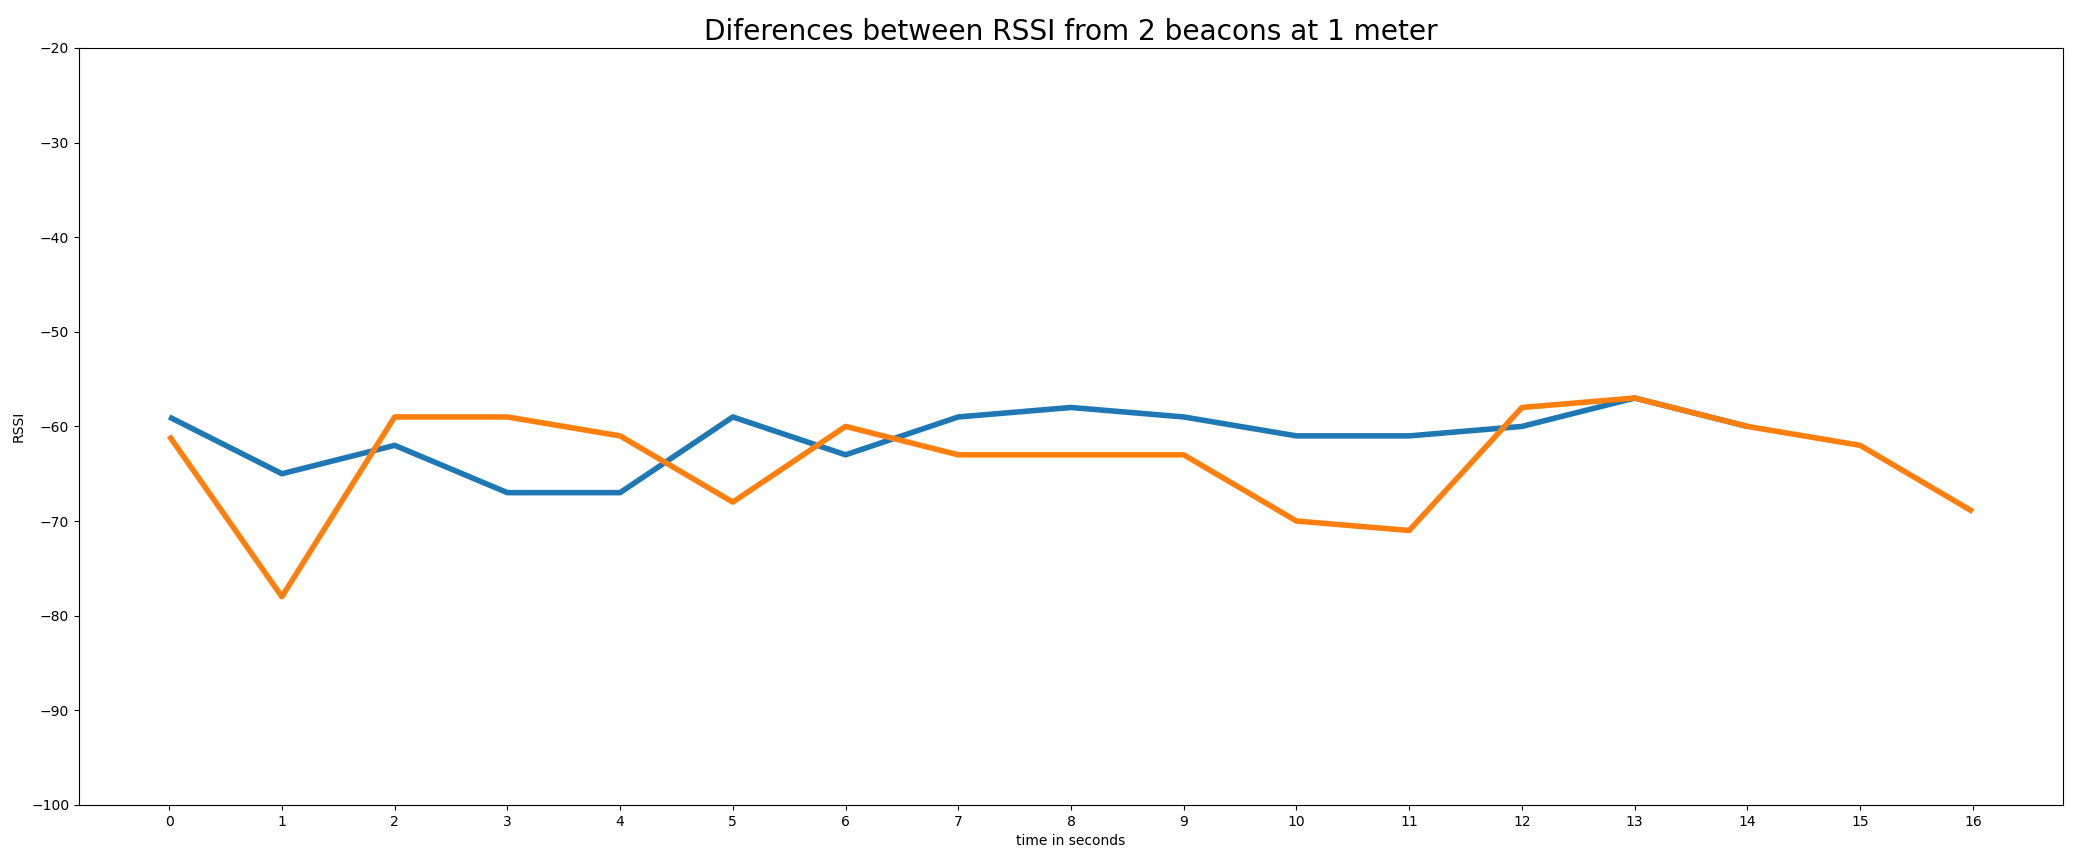
\includegraphics[scale=0.2]{10min_2beacons_same_distance.PNG}
                \end{center}
                Podemos ver de nuevo que las diferencias son notables, esto de nuevo afianza la idea de implementar
                un filtro que no falsee las medidas y cree falsas distancias puntuales entre los equipos.
                \paragraph{}
                El filtro más habitual para este tipo de aplicaciones es el denominado Kalman Filter:
                \begin{equation}
                    RSSI_suavizado=\alpha · RSSI_{n} + (1-\alpha) · RSSI_{(n-1)}
                \end{equation}
                Otra opción que experimentalmente me ha dado buenos resultados es la de coger lo 20 valores anteriores,
                obtener la media y si se separa más de un 30\% el valor nuevo lo rechazo. Con esto consigo eliminar las 
                fluctuaciones indesadas.
            \subsubsection{Trilateración y posicionamiento}
                Una vez obtenidas las distancias a los distintos equipos que receptores es necesario llevar a cabo el
                posicionamiento exácto de los equipos, para ello se emplea la trilateración:
                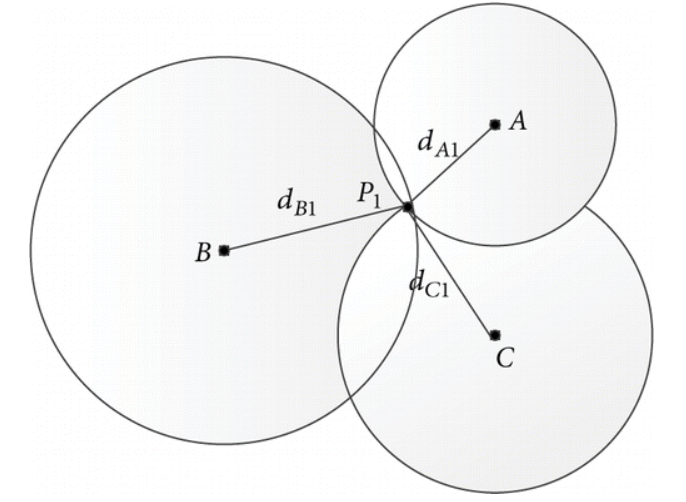
\includegraphics[scale=0.3]{trilateration_circle.png}
                Para ello hemos de resolver las siguientes ecuaciones básicas sobre la distancia entre recta y un punto en 
                    una circunferencia:
                    \begin{equation}
                        d_{A1}= \sqrt[2]{(x-x_A)^2+(y-y_A)^2}
                    \end{equation}
                    \begin{equation}
                        d_{B1}= \sqrt[2]{(x-x_B)^2+(y-y_B)^2}
                    \end{equation}
                    \begin{equation}
                        d_{C1}= \sqrt[2]{(x-x_C)^2+(y-y_C)^2}
                    \end{equation}
                    Llevando a cabo la simplificación obtenemos el siguiente sistema:
    \subsection{Cálculo de consumos energéticos}
            \begin{itemize}
                \item  Active Mode, 160-260mA.  Los dos cores del procesador encendidos así como el procesador ULP,
                RTC, Wifi, Bluetooth, Radio, Peripherals.
                \item  Sleep mode: 3-20mA Activos los dos cores, el coprocesaror ULP coprocessor y el RTC, inactivos el 
                Wifi, Bluetooth, Radio y periféricos.
                \item  Light sleep mode: La CPU está pausada apagando los pulsos de su reloj interno, sin embargo, el RTC
                y el coprocesador ULP se mantien activo. Esto supone consumo menor que en los anteriores modos de funcionamiento,
                se puede llegar a los 0.8mA.
                \item Deep sleep mode, tanto la CPU como gran parte de la RAM así como todos los periféricos se mantienen 
                apagados. Las únicas parte nos apagadas son los RTC de los periféricos y de la CPU (incluyendo el ULP) y su
                memoria interna. El chip consume en torno a los 0.15 mA si se mantien encendido el ULP y  10µA si no.
                En el modo deep sleep todo se encuentra apagado por ello los datos de la memoria del rtc se pierden
                puesto que se encuentra en reinicio el uP.
                \item Hibernation mode: A diferencia del modo deep sleep el oscilador de 8MHz y el ULP se encuentran apagados,
                no es posible almacenar nada de información. Tan solo el RTC funcinando con el reloj de baja velocidad puede funcionar.
                En este modo de funcionamiento el micro consume sobre los 2.5µA.
            \end{itemize}
            \begin{center}
                \begin{tabular}{||c || c ||} 
                \hline
                Modo del ESP32  & Consumo energético  \\ [0.5ex] 
                \hline
                Wi-Fi Tx a 13dBm~21dBm & 160~260mA  \\ 
                Wi-Fi/BT Tx  a packet 0dBm	 & 120mA  \\
                Wi-Fi/BT Rx and listening & 80~90mA  \\
                Sleep mode &  3-20mA   \\
                Light sleep mode &0,8mA  \\
                Deep sleep mode &   0,15 mA - 10µA  \\
                Hibernation mode & 2,5µA  \\
                \end{tabular}
            \end{center}
            A la hora de llevar a cabo la decisión sobre como llevar a cabo el protocolo de comunicación se ha de tener en cuenta 
            el consumo de los equipos, en especial en lo que respecta a los beacons.
            Es por ello por lo que se ha optado es por dormir el equipo durante 58 segundos, despertárlo,
            enviar su trama bluetooth y luego dormirlo hasta la siguiente vez que despierte.
            Con esto conseguimos un consumo que varía en función de la frecuencia de envio, en la siguiente tabla
            se puede ver un análisis en función del tiempo:
            \begin{center}
                \begin{tabular}{||c || c ||} 
                \hline
                Frecuencia de envio  & Consumo energético  \\ [0.5ex] 
                \hline
                1 min &  2,415 mA \\
                5 min &  0,495 mA \\ 
                10 min &  0,255 mA \\ 
                15 min &  0,175 mA \\ 
                30 min &  0,095 mA \\ 
                \hline
                \end{tabular}
            \end{center}
            Y en consecuencia está la duración media de las baterías, poniendo el ejemplo para una frecuencia de 
            envío de 10 minutos vemos que la autonomía será:
            \begin{center}
                \begin{tabular}{|c | c| c| c |} 
                \hline
                    Tipo de batería & Capacidad (mAh) & Autonomía(días) & Autonomía(días)   \\ [0.5ex] 
                    &  &  f=10 min &  f=5 min   \\ [0.5ex] 
                \hline
                \hline
                    Pila CRC 2032 &  240 mAh  & 39   & 20 \\ 
                    Pila AA       &  2500 mAh & 409  & 210 \\ 
                    Batería Li-Ion&  1600 mAh & 261  & 135 \\ 
                \hline
                \end{tabular}
            \end{center}
    \subsection{Cálculo saturación espectro de frecuencia}
            Los fundamentos básicos de las distintas frecuencias es que a menor frecuencia mayor distancia vamos a conseguir 
            en las comunicaciones. Por el contrario, cuanto menor frecuencia menor volumen de datos es posible.
            La tecnología bluetooth usa la frecuencia de 2.4GHz ISM (2400 to 2483.5 MHz), esta banda permite una buena relación
            de compromiso entre distancia y volumen de datos a transmitir.
            El espectro de frecuencia es amplio y cada banda tiene su aplicación, dentro de las telecomunicaciones
            distinguimos las siguientes opciones:
            \begin{itemize}
                \item Banda ISM: Son las bandas de radio industriales, científicas y médicas, están reservadas a 
                nivel internacional para estos usos y pueden usarse sin licencias por parte de gobiernos. El uso de esta
                banda conlleva que todo equipo emisor ha de estar protegido frente a interferencias dentro de su mismo 
                rango, es decir han de ser tolerantes a errores.
    
                Desde el microondas y el mando del garaje hasta el bluetooth, NFC y wifi son ejemplos de tecnologías
                que emplean este rango que se encuentra comprendido desde   6.78 MHz hasta 244 GHz en distintos tramos,
                un ejemplo de tramos serían los siguientes:
                \begin{center}
                    \begin{tabular}{||c | c | c| c ||} 
                    \hline
                    Rango de frecuencia & Bandwidth & Center Frequency & Allocation\\ [0.5ex] 
                    \hline
                    \hline
                        6.765 - 6.975 MHz &	0.03 MHz &	6.78 MHz	 & Locally \\ 
                        13.553 - 13.567 MHz &	0.014 MHz &	13.56 MHz	 & Global\\ 
                        26.957 - 27.283 MHz &	0.326 MHz &	27.18 MHz	 & Global\\ 
                        40.66 - 40.7 MHz &	0.04 MHz &	40.68 MHz	 & Global\\ 
                        433.05 - 434.79 MHz &	1.74 MHz &	433.92 MHz & EU, RU, Africa\\ 
                        902 - 928 MHz &	26 MHz&	915 MHz &	Americas\\   
                        2400 - 2500 MHz &	100 MHz &	2450 MHz & Global\\ 
                        5725 - 5875 MHz &	150 MHz &	5800 MHz & Global\\ 
                        24 - 24.250 GHz &	250 MHz &	24.125 GHz & 	Global\\ 
                        61 - 61.5 GHz &	500 MHz &	61.250 GHz & 	Locally \\ 
                        122 - 123 GHz &	1000 MHz &	122.5 GHz	 & Locally \\ 
                        244 - 246 GHz &	2000 MHz &	245 GHz & Locally \\ 
                    \hline
                    \end{tabular}
                \end{center}
                \item Banda no ISM: Para usos no licenciados: Son aquellas que no requieren permisos especiales de las 
                autoridades para su uso. A nivel mundial el 2,4GHz está dentro de las frecuencias de libre utilización 
                con ciertas limitaciones en algunos paises.

                Es por ello por lo que al ser libres podemos tener emitiendo a nuestros equipos sin preocuparnos por
                la legislación existente, la gran versatilidad para tranmitir también conlleva un mayor número de equipos 
                en este ancho de banda y mayores dificultades.
            \end{itemize}
            La frecuencia de 2.4 GHz con su estándar 802.11 b/g/n ha llegado al límite de su capacidad, se han
            detectado incluso caidas del 30\% en areas urbanas.  
            La banda ISM de 2.4GHz es, sin lugar a dudas, la que soporta un uso más intensivo, ya que es utilizada en 
            diferentes estándares de redes Wi-Fi (IEEE 802.11b/g/n) y Bluetooth, (IEEE 802.15.1), llegando en muchas 
            ocasiones a su completa saturación.
    \subsection{Cálculo de ganancia de antenas}
            Una antena convierte la enegía electrica del transmisor en energía electromagnética y viceversa, las antenas pueden ser 
            para recibir, para transmitir o ambas. La localización de la antena, las dimensiones y el diseño pueden afectar drásticamente
            en el funcionamiento óptimo de la red de beacons. 
            Las antenas típicas en aplicaciones de radiofrecuencia con bluetooth son de -10dBm a 10dBm.

            El denominado path loss o atenuación de la señal de radio es la reducción de la densidad de potencia de una onda durante la 
            propagación en el espacio. Este parámetro es esencial a la hora de poder establecer una red de bluetooth de estas dimensiones.
            Antenas monopolo $\lambda$/4
            Antenas dipolo $\lambda$ /2 
            \paragraph{}
            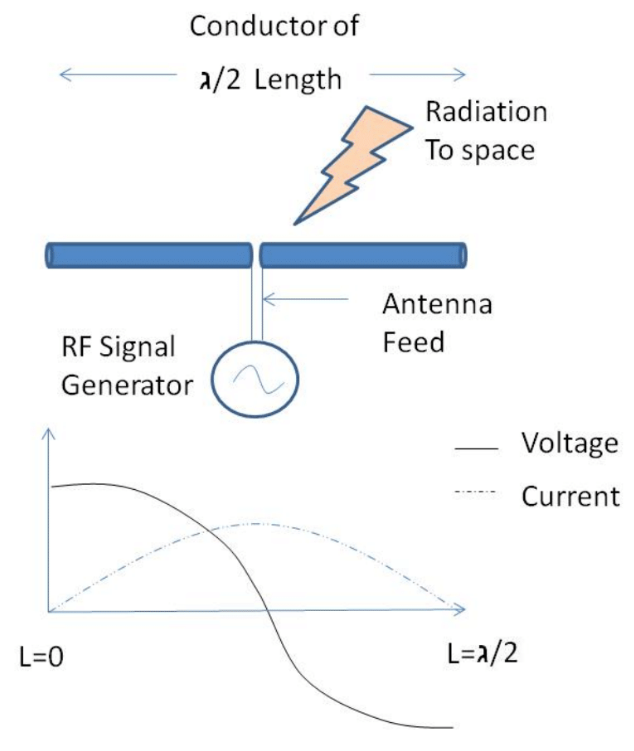
\includegraphics[scale=0.4]{antenna_design.png}
            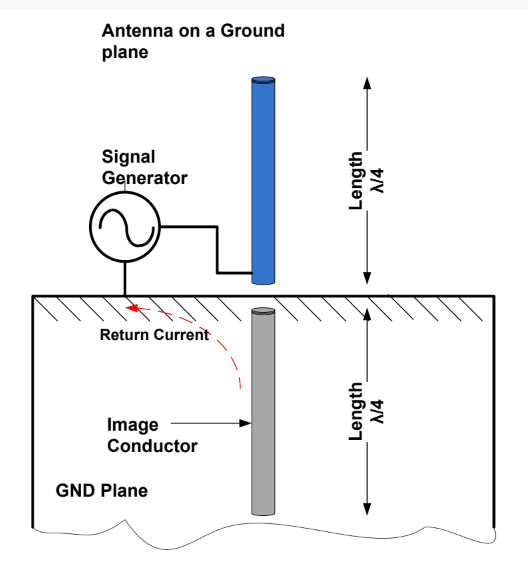
\includegraphics[scale=0.5]{antenna_design_monopole.png}
            \paragraph{}
            Dentro del mundo de las antenas existen numerosos modelos u opciones que se enumeran a continuación:
            \begin{enumerate}
                \item Antenas de cable, son las más sencillas de todas y como su propio nombre indica es un simple cable soldado a la PCB de una dimensión determinada, esta logitud corresponde con la de una antena monopolo $\lambda$/4. El cable aporta el mayor rendimiento y rango de radiofrecuencia debido a sus dimensiones y a su caracter flexible, moldeable y orientable sin importar  la posición de la tarjeta.
                \item Antena PCB, es una pista en el propio circuito impreso que puede tener numerosas formas, a diferencia de la de cable esta solo se encuentra en el espacio 2D. Tienen menos eficiciencia que las anteriores y requieren más espacio pero son incluso más baratas.
                \item Antena de chip, este tipo de antena es una tarjeta o módulo que ocupa menos espacio que cualquiera de las anteriores y tiene un rendimiento intermedio entre ambas otras dos opciones.
            \end{enumerate}
\section{Planos}
    \subsection{Planos mecánicos}
        \subsubsection{Chasis de receptor o gateway}
        \subsubsection{Chasis de emisor o beacon}
    \subsection{Plano eléctricos}
        \subsubsection{Esquemático del emisor beacon}
        \subsubsection{PCB circuito del emisor beacon}
        \subsubsection{Esquemático del receptor ESP32}
        \subsubsection{PCB circuito del receptor ESP32}
\section{Pliego de condiciones}
    \subsection{Prescripciones ténicas generales}
    \subsubsection{Normativa relativa a radiofrecuencia}
    \subsubsection{Normativa relativa a bluetooth}
    Se ha de tener en cuenta que para poder emplear dispositivos bluetooth se ha de respetar los estándares
    \begin{itemize}
        \item IEEE 802.15.1 define Bluetooth 1.x, que puede alcanzar velocidades de 1 Mbps;
         \item IEEE 802.15.2 recomienda prácticas para utilizar la banda de frecuencia de 2.4 GHz (la frecuencia también utilizada por WiFi). Sin embargo, este estándar todavía no se ha aprobado;
         \item IEEE 802.15.3 es un estándar que actualmente se está desarrollando, que ofrecerá velocidad de banda ancha (20 Mbps) con Bluetooth;
         \item IEEE 802.15.4 es un estándar que actualmente se está desarrollando para el uso con aplicaciones Bluetooth de baja velocidad.
    \end{itemize}
    Se ha de tener en cuenta también la clase del disposivo que queda recogida en la siguiente tabla:
    \begin{center}
        \begin{tabular}{||c | c |c ||} 
        \hline
        Clase & Potencia  & Alcance aproximado\\ [0.5ex] 
        \hline\hline
        Clase 1 & 100 mW / 20 dBm & 100 m \\ 
        Clase 2 & 2,5 mW / 4 dBm & 5 - 10 m \\ 
        Clase 3 & 1 mW / 0 dBm & 1 m \\ 
        Clase 4 & 0,5 mW / -3 dBm & 0,5 m \\ 
    \hline
        \end{tabular}
    \end{center}
    En nuestro caso y teniendo en cuenta la aplicación se ha optado por emitir en los 20 dBm de tal forma
    que se ha de 
    \subsection{Prescripciones ténicas particulares}
        \subsubsection{Condiciones que ha de reunir el material}
        \subsubsection{Ejecución del proyecto}
        Placa ha de cumplir solo 1 capa
\section{Presupuestos}
    \subsection{Precios unitarios}
        La tabla de precios se va a elaborar en distintas unidades que corresponden al precio por separado de cada
        una de las PCBs que se han elaborarado.
    \subsection{Presupuestos Parciales}
            \subsubsection{Placa de circuito impreso emisor beacon}
                \begin{center}
                    \begin{tabular}{||c | c |c ||} 
                    \hline
                    Componente & Cantidad & Precio unitario  \\ [0.5ex] 
                    \hline
                    Resistencia metálica SMD 0805 1k 10  	&1&	 0,009 € \\ 
                    Resistencia metálica SMD 0805 10k 10 	&1&	 0,009 € \\ 
                    Condensador cerámico SMD 0805 0,1uF  	&1&	 0,005 € \\ 
                    Condensador cerámico SMD 0805 10uF   	&1&	 0,016 € \\ 
                    Regulador tensión LDO AMS1117-3.3V   	&1&	 0,098 € \\ 
                    Microcontrolador ESP32-WROOM-32D     	&1&	 2,840 € \\ 
                    Led SMD 0805 verde                   	&1&	 0,013 € \\ 
                    Led SMD 0805 rojo                    	&1&	 0,013 € \\ 
                    Led SMD 0805 naranja                 	&1&	 0,015 € \\ 
                    Batería Litio Ion                    	&1&	 1,520 € \\ 
                    \hline
                    TOTAL                    	            &1&	 4,009 € \\ 

                \hline
                    \end{tabular}
                \end{center}
            \subsubsection{Placa de circuito impreso receptor o gateway}
                \begin{center}
                    \begin{tabular}{||c | c |c ||} 
                    \hline
                    Componente & Cantidad & Precio unitario  \\ [0.5ex] 
                    \hline
                    Resistencia metálica SMD 0805 1k 10  	&1&	 0,009 € \\ 
                    Resistencia metálica SMD 0805 10k 10 	&1&	 0,009 € \\ 
                    Condensador cerámico SMD 0805 0,1uF  	&1&	 0,005 € \\ 
                    Condensador cerámico SMD 0805 10uF   	&1&	 0,016 € \\ 
                    Regulador tensión LDO AMS1117-3.3V   	&1&	 0,098 € \\ 
                    Microcontrolador ESP32-WROOM-32D     	&1&	 2,840 € \\ 
                    Led SMD 0805 verde                   	&1&	 0,013 € \\ 
                    Led SMD 0805 rojo                    	&1&	 0,013 € \\ 
                    Led SMD 0805 naranja                 	&1&	 0,015 € \\ 
                    Pinheader conector para programación 	&1&	 0,113 € \\ 
                    UART-TTL herramienta de dasarrollo   	&1&	 1,540 € \\ 
                    Power Module AC-DC HI-LINK 3.3V	        &1&	 2,830 € \\ 
                    Screw terminal P=5.08mm	                &1&	 0,097 € \\ 
                    USB Mini B Female                    	&1&	 0,108 € \\ 
                    JST Connector P=2mm                  	&1&	 0,039 € \\ 
                    Jumper connector	                    &1&	 0,017 € \\ 
                    \hline
                    TOTAL                    	            &&	 7,763 € \\ 
                    \end{tabular}
                \end{center}
            \subsubsection{Desarrollo e instalación}
            \begin{center}
                \begin{tabular}{||c | c |c ||} 
                \hline
                Componente & Cantidad (h) & Precio unitario  \\ [0.5ex] 
                \hline\hline
                Diseñador hardware placas circuito impreso   & 10  & 50 \\ 
                Desarrollador  software sistema embebido     & 350 & 40 \\ 
                Programador full stack web developer         & 100 & 50 \\ 
                Instalador de equipos, oficial de 1ª         & 2   & 35 \\ 
                \hline
                \end{tabular}
            \end{center}
    \subsection{Presupuestos Total}
        El presupuesto total se compone de la suma de los presupuestos parciales:
        \begin{center}
            \begin{tabular}{||c | c |c ||} 
            \hline
            Unidad & Cantidad & Precio  \\ [0.5ex] 
            \hline\hline
            Placa de circuito impreso beacon o emisor & 1 & 40 \\ 
            Placa de circuito impreso receptor o gateway & 1 & 50 \\ 
            Desarrollo e instalación & 1 & 35 \\ 
            \hline
            \hline
            Total &  & 1234€ \\ 
             & IVA 21\%& 6534€ \\ 
             & & 6534€ \\ 
            \hline
            \end{tabular}
        \end{center}
        Por lo tanto el presupuesto total con iva asciende a la cantidad de 1234123 4123 y veintimeil euros.
    \subsection{Factores económicos y financieros}
    Estudio de viabilidad económica
        \subsubsection{Tasa de interés de retorno(TIR)}
        \subsubsection{Valor Actual Neto (VAN)}

\section{Bibliografía}
- https://www.bluetooth.com/
- https://accent-systems.com/es/producto/ibks-105/
\end{document} 